\documentclass[margin=16pt]{standalone}
\usepackage{tikz}
\usetikzlibrary{arrows}

\tikzset{
    >=stealth' % Default arrow tip 
}

\tikzstyle{every node}=[
    draw,
    circle,
    fill = black,
    inner sep = 0cm,
    minimum width = 0.12cm
]


\begin{document}
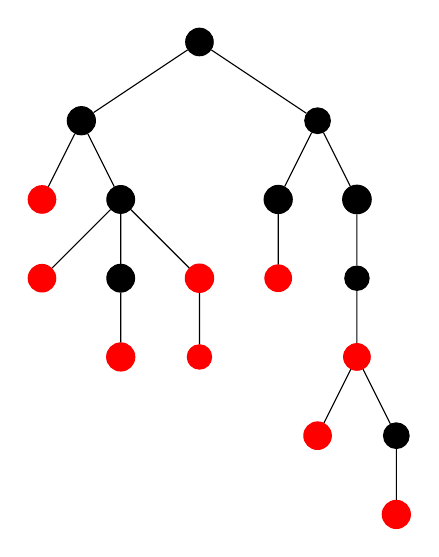
\begin{tikzpicture}[level distance=10mm]
    \tikzstyle{level 1}=[sibling distance=30mm]
    \tikzstyle{level 2}=[sibling distance=10mm]

    \node {C}
        child {node {A}
            child {node [red] {T}}
            child {node {R}
                child {node [red] {T}}
                child {node {R}
                    child {node [red] {Y}}
                }
                child {node [red] {D}
                    child {node [red] {S}}
                }
            }
        }
        child {node {L}
            child {node {U}
                child {node [red] {E}}
            }
            child {node {O}
                child {node {S}
                    child {node [red] {E}
                        child {node [red] {T}}
                        child {node {L}
                            child {node [red] {Y}}
                        }
                    }
                }
            }
        }
    ;
\end{tikzpicture}
\end{document}


%
%```plantuml
%@startdot
%
%graph a {
%    node [shape=plaintext]
%    "*" [label="*" ]
%    "*1" [label="*" shape=point]
%    "*2" [label="*" shape=point]
%    "*3" [label="*" shape=point]
%    "*4" [label="*" shape=point]
%    "*5" [label="*" shape=point]
%    "*6" [label="*" shape=point]
%    "*7" [label="*" shape=point]
%    "*8" [label="*" shape=point]
%    "*9" [label="*" shape=point]
%    "*10" [label="*" shape=point]
%
%    "*" -- {C T}
%    C -- {CA CO}
%    CA -- CAR
%    CAR -- {"*1" CARD}
%    CARD -- {"*2" CARDS}
%    CARDS -- "*3"
%    CO -- COT
%    COT -- {"*4" COTS}
%    COTS -- "*5"
%    T -- TR
%    TR -- {TRI TRY}
%    TRY -- "*6"
%    TRI -- {TRIE, TRIM}
%    TRIM -- "*7"
%    TRIE -- {"*8" TRIED TRIES}
%    TRIED -- "*9"
%    TRIES -- "*10"
%}
%
%@enddot
%```
